\documentclass{beamer}

\usepackage[orientation=portrait,size=a0,scale=1.1]{beamerposter}
\usepackage{graphicx}
\usepackage{xcolor}
\usepackage{ragged2e}

% --- Specific Blue theme ---
\definecolor{maincolour}{RGB}{94, 114, 197}
\definecolor{darkercolour}{RGB}{7, 26, 99}
\setbeamercolor{title}{fg=white,bg=maincolour!70}
\setbeamercolor{block title}{fg=white,bg=maincolour!70}
\setbeamercolor{block body}{fg=black,bg=maincolour!5}

%Create Divider
\newcommand{\divider}{
	\vspace{1cm}
	\noindent\color{maincolour}\rule{\linewidth}{7pt}
	\vspace{0.5cm}
}

\newcommand{\sectiontitle}[1]{
	\vspace{0.5cm}
	{\LARGE\color{maincolour}\textbf{#1}}
	\vspace{0.5cm}
}


\title{\VeryHuge Where is the UK in the AI race?}
\author{Ellen Beattie}
\institute{Source: Global Artificial Intelligence Indicator Database (GAID) 1998-2025, sourced from the \href{https://dataverse.harvard.edu/dataset.xhtml?persistentId=doi:10.7910/DVN/QYLYSA}{Harvard Dataverse}} 

\begin{document}
	
	\begin{frame}[t]
		
	% --- Title bar ---
	\begin{beamercolorbox}[wd=\paperwidth,ht=5cm,center]{title}
		{\VeryHuge \textbf{\inserttitle}}\\[0.5cm]
		{\Large \insertauthor \hspace{1cm} \insertinstitute}
	\end{beamercolorbox}
			
			\vspace{2cm}
			
	% ================= SECTION 1 =================
	\sectiontitle{Economic Vibrancy}
	
	\vspace{0.7cm}

	\begin{columns}
		\begin{column}{0.495\textwidth}
			\begin{minipage}{0.95\linewidth}
				
				\centering
				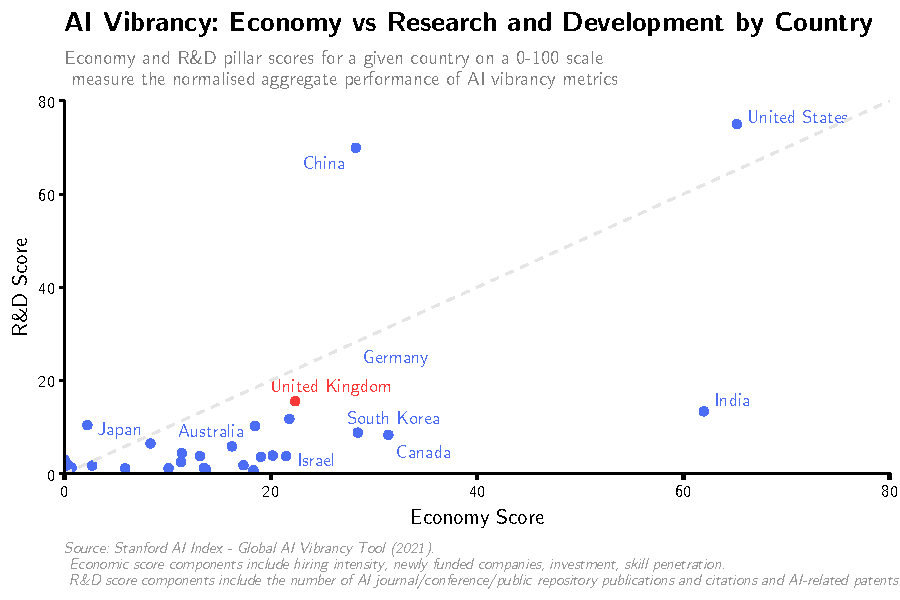
\includegraphics[width=\linewidth]{figures/figure1.pdf}
				
				\vspace{0.3cm}
				\justifying
				{\large\color{darkercolour}
					  When it comes to AI vibrancy in the Economy (capacity to exploit AI) and Research and Development (innovation capacity), the UK is one of the leaders of the chasing pack below the US, China and India.}
				
			\end{minipage}
			
		\end{column}
		
		
		\begin{column}{0.495\textwidth}
			\begin{minipage}{0.95\linewidth}
				
				\centering
				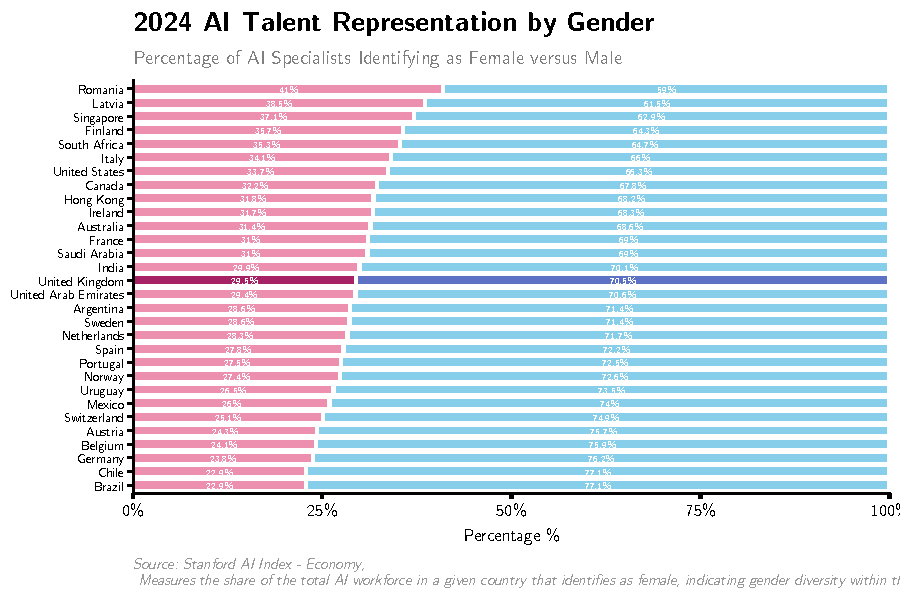
\includegraphics[width=\linewidth]{figures/figure3.pdf}
				
				\vspace{0.3cm}
				\justifying
				{\large\color{darkercolour}
						Women are under-represented in the AI workforce with only 29.5\% of the UK AI specialists being female, which is broadly typical of a global issue of gender inequality in AI talent}
				
			\end{minipage}
			
		\end{column}
	\end{columns}
	
	\divider
	
	% ================= SECTION 2 =================
	\sectiontitle{Public Opinion}
	
	\vspace{0.7cm}
	
	\begin{columns}
		\begin{column}{0.495\textwidth}
			\begin{minipage}{0.95\linewidth}
				
				\centering
				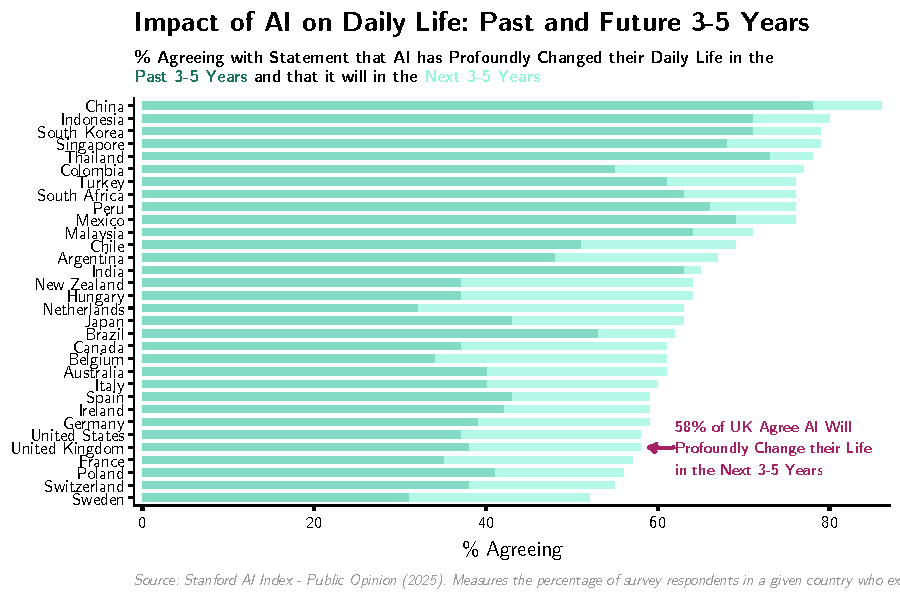
\includegraphics[width=\linewidth]{figures/figure4.pdf}
				
				\vspace{0.3cm}
				\justifying
				{\large\color{darkercolour}
					Fewer people in the UK have felt that their life has been or will be drastically changed by AI compared with most other countries. China, Indonesia and South Korea lead as having the greatest percentage of people reporting and anticipating profound change to their daily lives because of AI.}
				
			\end{minipage}
			
		\end{column}
		
		
		\begin{column}{0.495\textwidth}
			\begin{minipage}{0.95\linewidth}
				
				\centering
				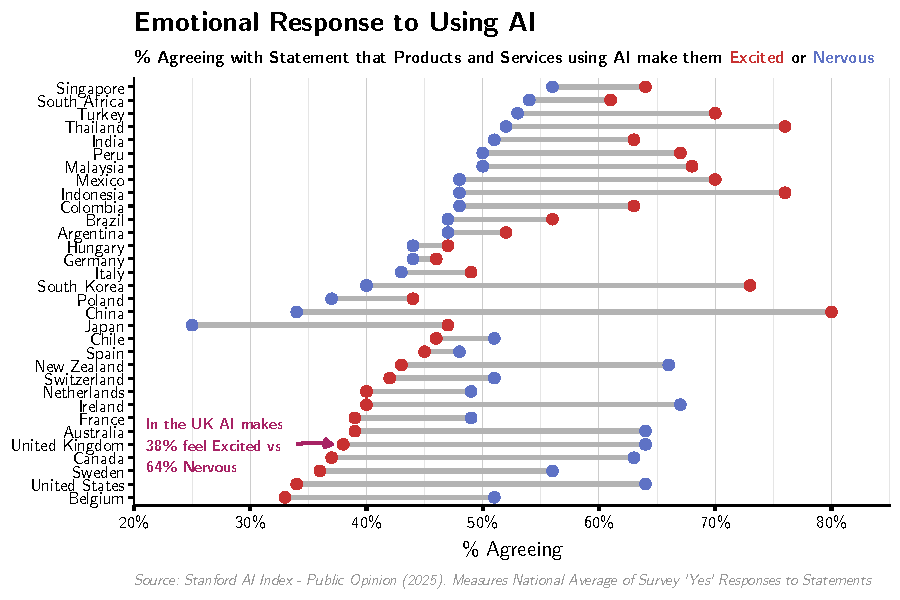
\includegraphics[width=\linewidth]{figures/figure5.pdf}
				
				\vspace{0.3cm}
				\justifying
				{\large\color{darkercolour}
					A substantially higher proportion of the UK public feel more nervous than excited about AI use, a trend seen across other European and North American nations. In other countries, especially those in Asia and South America, more people feel excited and less nervous about AI use.}
				
			\end{minipage}
			
		\end{column}
	\end{columns}
	
	\divider
	
	% ================= SECTION 3 =================
	\sectiontitle{Ethics and Responsible AI practices}
	
	\vspace{0.7cm}
	
	\begin{columns}
		\begin{column}{0.495\textwidth}
			\begin{minipage}{0.95\linewidth}
					
			\centering
			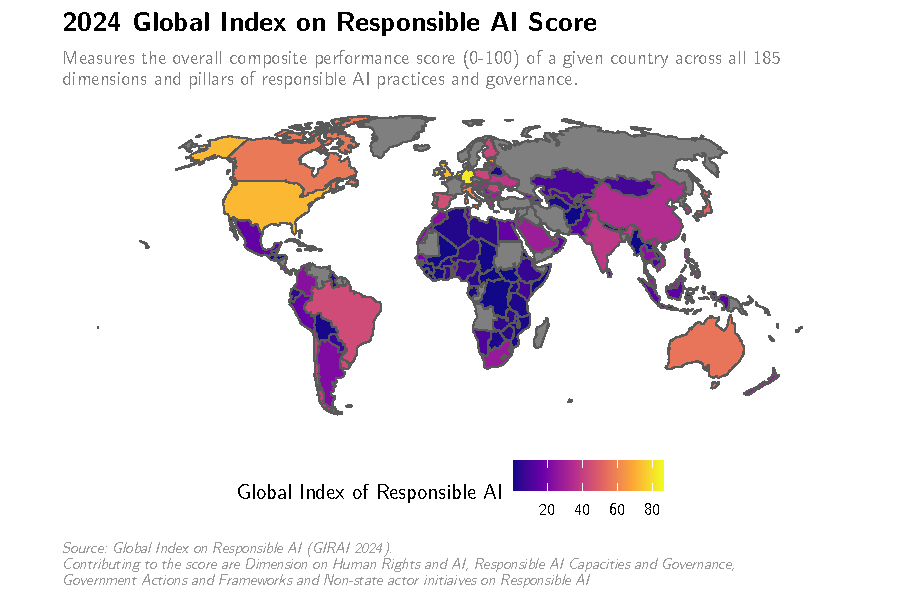
\includegraphics[width=\linewidth]{figures/figure6.pdf}
			
			\vspace{0.3cm}
			\justifying
			{\large\color{darkercolour}
				Western nations are leading globally as the most responsible in terms of AI practises and governance, with lower scores across South America, Africa and Asia. The UK falls just behind Germany and the Netherlands indicating they are enacting responsible AI initiatives, frameworks and policy to a reasonable extent.}
			
			\end{minipage}
			
		\end{column}
		

		\begin{column}{0.495\textwidth}
			\begin{minipage}{0.95\linewidth}
				
				\centering
				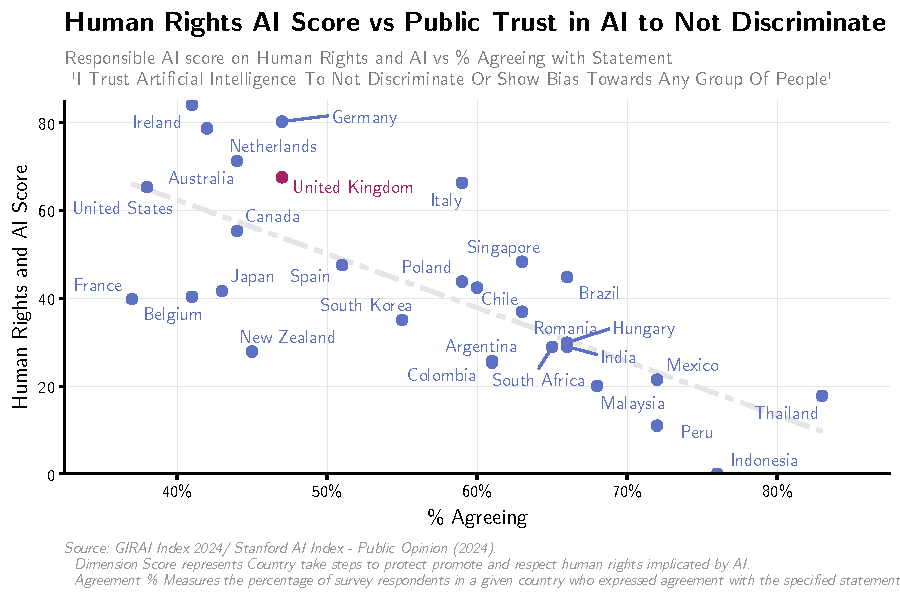
\includegraphics[width=\linewidth]{figures/figure7.pdf}
				
				\vspace{0.3cm}
				\justifying
				{\large\color{darkercolour}
					The UK has a moderately high Human Rights and AI score ($>$60) yet a less then half of the public surveyed said that they trusted AI to not discriminate or show bias. This is consistent with a general negative relationship between a higher public trust in AI to be non-discriminatory, and a lower human rights and AI score.}
				
			\end{minipage}
			
		\end{column}
	\end{columns}



\end{frame}


	
\end{document}
